\documentclass[11pt,fleqn]{article} 
\usepackage[margin=0.8in, head=0.8in]{geometry} 
\usepackage{amsmath, amssymb, amsthm}
\usepackage{fancyhdr} 
\usepackage{palatino, url, multicol}
\usepackage{graphicx} 
\usepackage[all]{xy}
\usepackage{polynom} 
\usepackage{pdfsync}
\usepackage{enumerate}
\usepackage{framed}
\usepackage{setspace, adjustbox}
\usepackage{array%,tikz, pgfplots
}

\usepackage{tikz, pgfplots}
\usetikzlibrary{calc}
%\pgfplotsset{my style/.append style={axis x line=middle, axis y line=
%middle, xlabel={$x$}, ylabel={$y$}, axis equal }}
%
\pagestyle{fancy} 
\lfoot{UAF Calculus I}
\rfoot{4-2}


\newcommand{\be}{\begin{enumerate}}
\newcommand{\ee}{\end{enumerate}}

\newcommand{\bi}{\begin{itemize}}
\newcommand{\ei}{\end{itemize}}

\begin{document}
\setlength{\parindent}{0cm}
\renewcommand{\headrulewidth}{0pt}
\newcommand{\blank}[1]{\rule{#1}{0.75pt}}
\renewcommand{\d}{\displaystyle}
\vspace*{-0.7in}
\begin{center}
 {\large{ \sc{Section 4.2: Linear Approximations and Differentials}}}
\end{center}
 \begin{enumerate}
 \item The linear approximation, $L(x)$, of $f(x)$ at $x=a$ is: 
 \vspace{.5in}
 \item Let $f(x)=x^{4/3}.$ 
 %\begin{multicols}{2}
 	\begin{enumerate}
	\item Find the linear approximation $L(x)$ of $f(x)$ at $a=1.$
	\vfill
	\item Sketch $L(x)$ on the graph below.\\
	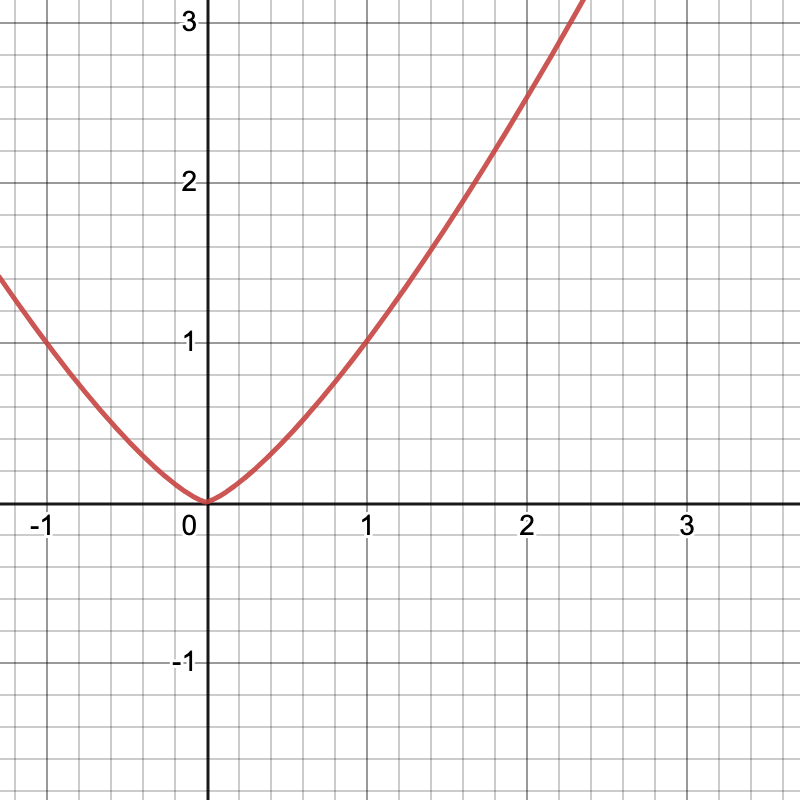
\includegraphics[scale=.2]{4-2-pic.png}
	
	\item Use $L(x)$ to estimate $(1.1)^{4/3}$ and mark this y-value on the graph above.
	\vfill
	\item Use your calculator to find $(1.1)^{4/3}$ exactly, mark this y-value on the graph above, determine the error between the exact value and the estimate, and mark the error on the graph above.
	\vfill
	\end{enumerate}
\item Estimate $\frac{1}{2.01}$ using an appropriate linear approximation (pick an $f(x)$ and an $a$). Use your calculator to determine the exact value and the error.\vfill
\newpage
\item The differential of $y=f(x)$ is 
\vspace{.5in}
\item Given $f(x)=x \sin( \frac{\pi}{2} x)$. 
	\begin{enumerate}
	\item Find the differential of $f(x)$ and evaluate the differential when $x=2$ and $dx=0.1.$
	\vfill
	\item Use a calculator to find $f(2.1)-f(2).$
	\vfill
	\item Explain what the calculations in parts (a) and (b) represent and why they are close but not the same.
	\vfill
	\end{enumerate}
\item The side of a cube is measured to be 2 meters with a possible error in measurement of $0.1$ meter. Use differentials to estimate the maximum possible error when computing the volume of the cube. Determine the relative (or percent) error.
\vfill
%\end{multicols}
\end{enumerate}
\end{document}